\chapter{Stellarators}
\section{Historia y precedentes}
El concepto \textit{stellarator} se debe al astrofísico Lyman Spitzer~\cite{doi:10.1063/1.1705883}, quien lo
introdujo en 1951. Algunos años más tarde se construyó en Princeton el primer experimento de confinamiento con \textit{stellarator} llamado modelo C, pero
no tuvo éxito: el plasma se perdía muy rápidamente es decir, sus tiempos
de confinamiento eran mucho menores de lo esperado. Como se entendería
luego, esto se debía principalmente a un conocimiento incompleto sobre el
comportamiento de las resonancias en las superficies magnéticas. Mientras
el experimento del \textit{stellarator} de Princeton carecía todavía de un buen confinamiento (solo unos pocos tiempos de Bohm2~\footnote{El tiempo Bohm es $\tau_B=\frac{a^2}{D_B}$, $a$ es el radio menor y el coeficiente de difusión de Bohm es $D_B=\frac{1}{16}\frac{k_BT_e}{eB}$, donde $B$ es el campo magnético, $T_e$ es la temperatura electrónica, $e$ es la carga elemental y $k_B$ es la constante de Boltzmann.}
a $T_e\approx100 eV$) los científicos
rusos presentaban en la conferencia de Novosibirsk IAEA 1968~\cite{Artsimovich1969}, un concepto de confinamiento llamado \textit{tokamak}, con el cual era posible alcanzar
temperaturas electrónicas alrededor de 1 keV para 30 tiempos Bohm (varios
milisegundos).\par
Esta situación dio lugar al hecho histórico de que los \textit{tokamak} se convirtieron en la principal línea de investigación para la fusión nuclear por
confinamiento magnético, mientras que el concepto de \textit{stellarator} se desarrolló solo en algunos lugares, principalmente en el \textit{Max-Planck-Institut fur
Plasmaphysik} (IPP) en Garching y en la Universidad de Kyoto. Hoy en día
se ha renovado el interés en el concepto de \textit{stellarator} como alternativa al
\textit{tokamak}: un gran \textit{stellarator} tipo torsatrón llamado \textit{Large Helical Device}
(LHD) inició su operación en 1998 en Japón. También se está construyendo
en Alemania el \textit{stellarator} Wendelstein 7-X. En Estados Unidos de América
se está planeando un nuevo experimento llamado \textit{National Compact Stellarator Experiment} (NCSX). Otros \textit{stellarators} de tamaño medio están en uso en
Estados Unidos de América (HSX), en España (TJ-II) y en Australia (H-1).\par
\textit{Stellarator} es el nombre general para los dispositivos que confinan un plasma de fusión por medio de un campo magnético generado completamente por
bobinas externas. Por lo tanto, los \textit{stellarators} no necesitan corriente neta toroidal en el plasma para el confinamiento, y con la llegada de poderosas
fuentes auxiliares de calentamiento en la década de 1970 se logró que los \textit{stellarator} no requirieran corriente en el plasma para calentamiento óhmico. A
día de hoy, los \textit{stellarators} se calientan por resonancia ciclotrónica electrónica
(ECRH), por resonancia ciclotrónica iónica (ICRH\footnote{Del inglés \textit{Ion Cyclotron Resonance Heating}}), por inyección de haces
de neutros (NBI\footnote{Del inglés \textit{Neutral Beam Injection}}) y por combinación de estos métodos.\par
En ausencia de una gran corriente en el plasma, un \textit{stellarator} tiene una
inherente capacidad de funcionamiento en estado estacionario y no hay riesgos de fuertes inestabilidades debidas a la corriente, como por ejemplo las
disrupciones. Más allá de estas ventajas evidentes los \textit{stellarators} tienen que
demostrar su potencial como futuros reactores, cumpliendo los requisitos de
alta $\beta$ de operación~\ref{eq:beta}
(requerida por motivos económicos), alto confinamiento (requerido
para alcanzar la ignición) y un exhaustivo control del escape de potencia y
partículas (necesarios para control de densidad, y transferencia térmica).
\section{Conceptos fundamentales de un \textit{stellarator}}
El uso de los campos magnéticos externos ofrece una gran libertad para
realizar el confinamiento magnético: la formación de superficies magnéticas
anidadas y cerradas toroidalmente por el giro helicoidal de las líneas de campo
magnético es un requisito esencial para el confinamiento del plasma por un
campo magnético. Entendemos una superficie magnética o superficie de flujo
como aquella región del espacio donde, para un campo magnético dado $B(r)$,
existe una función $\Psi(r)$ tal que $B\cdot\nabla\Psi=0$ por lo que $\Psi(r)=constante$ en la
superficie (el campo magnético es tangente a estas superficies). La superficie de flujo más interna, la cual degenera
en una línea, se llama eje magnetico. Justamente las superficies magnéticas
son las que se utilizan para definir el sistema de coordenadas o coordenadas
magnéticas $(\Psi_t,\theta,\varphi)$ que permiten simplificar la forma funcional que describe
las líneas de campo magnético y separar la dirección perpendicular y paralela
más fácilmente~\cite{doi:10.1063/1.872833}. Aquí, $\Psi_t$ es el flujo toroidal encerrado por una superficie
magnética (normalmente se utiliza la coordenada radial $r\propto\sqrt\Psi_t$), $\theta$ es el
ángulo poloidal, y $\varphi$ es el ángulo toroidal. Todo esto permite especificar una
línea de campo en una superficie magnética como una función de la forma 
$\theta=f(\varphi)$ de tal manera que si $\varphi$ aumenta $2\pi n\;(n\in\mathbb{N})$ el ángulo $\theta$ (en radianes)
cambia una cantidad $\theta_n$. La cantidad $\iota$ definida en~\ref{eq:transrot} tiene el mismo valor para cada línea de
campo en una superficie de flujo dada.
\begin{figure}
    \centering
    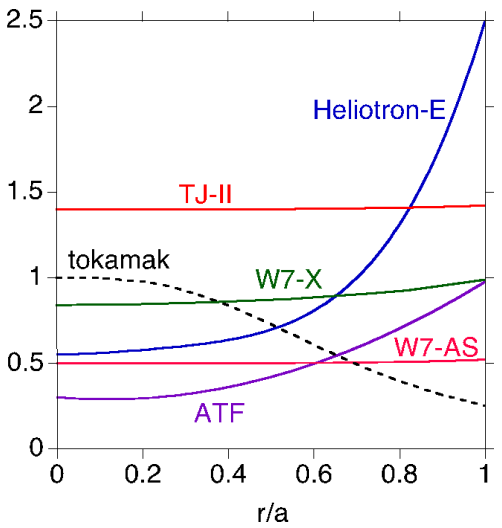
\includegraphics[scale=0.5]{img/compare.png}
    \caption[Perfiles radiales de transformada rotacional]{Perfiles radiales de transformada rotacional para diferentes
    conceptos de \textit{stellarators} y un \textit{tokamak}.}
    \label{fig:compare}
\end{figure}
Históricamente, los \textit{tokamaks} han utilizado el factor de seguridad $q=1/\iota$ y los stellarators $\iota$. En la figura~\ref{fig:compare} se muestran algunos perfiles de
transformada rotacional para diferentes \textit{stellarators} y un \textit{tokamak}. En un
\textit{tokamak} la corriente de plasma toroidal y por lo tanto su contribución al 
campo magnético poloidal decrece con la distancia al centro; así la rotación
de las líneas de campo decrece. En un \textit{stellarator} el campo magnético poloidal
aumenta con la distancia al centro porque la contribución de las bobinas
exteriores helicoidales aumenta.\par
La cizalla magnética dada por 
\begin{equation}\label{eq:cizalla}
    s=-\frac{\rho}{\iota}\frac{d\iota}{d\rho}
\end{equation}
donde $\rho$ es radio normalizado efectivo del reactor, describe la variación
radial de la rotación de las líneas de campo magnético. Es obvio en la figura~\ref{fig:compare} que los \textit{stellarators} y los \textit{tokamak} tienen signos opuestos de cizalla. Se
ha demostrado que las descargas de tokamak en las que se fuerza una cizalla
invertida, es decir, localmente este tipo de descargas tienen el mismo signo
de cizalla que un stellarator~\cite{PhysRevLett.75.4417}, a menudo tienen propiedades
de confinamiento mejorado en el plasma. TJ-II y W7-AS son \textit{stellarators}
con baja cizalla, mientras que LHD tiene una fuerte cizalla. Los
dispositivos con cizalla magnética tienen superficies de flujo con transformada
rotacional $\iota=n/m$, con $n$ y $m$ números naturales, llamados nómero toroidal
y número poloidal respectivamente. Este tipo de superficies de flujo se llaman
superficies racionales. Cuando m y n tienen valores pequeños, se
suelen llamar superficies racionales de bajo orden o simplemente racionales
de bajo orden. A modo de ejemplo, la superficie racional $\iota=8/5$,
se interpretaría geométricamente como: por cada $n=8$ vueltas poloidales la
línea de campo magnético daría $m=5$ vueltas toroidales. En una superficie
racional todas las líneas de campo son cerradas mientras que en una superficie
no racional las líneas de campo llenan la superficie magnética.
Existen inestabilidades que pueden producir que estas superficies
se destruyan localmente, dando origen a las llamadas islas magnéticas, esto son regiones del plasma donde las líneas llenan un volumen en vez de una
superficie y se hablara de ellas más adelante en este texto.